%\documentclass[12pt,draft]{article}
\documentclass[12pt]{article}
\usepackage{amsmath}
\usepackage{amsfonts}
\usepackage{times}
\usepackage{graphicx}
\usepackage{color}
\usepackage{multirow}
%
\usepackage[authoryear]{natbib}
%
\usepackage{rotating}
\usepackage{bbm}
\usepackage{latexsym}
%\DeclareGraphicsExtensions{.eps,.png}

% reference links
\usepackage{nameref,hyperref}
\usepackage[table]{xcolor}
\hypersetup{
    colorlinks = true,                    % text and not border
    citecolor = {teal},
    linkcolor = {purple},
           }
% black, blue, brown, cyan, darkgray, gray, green, lightgray, lime, 
% magenta, olive, orange, pink, purple, red, teal, violet, white, yellow.

%%% margins 
\textheight 23.4cm
\textwidth 14.65cm
\oddsidemargin 0.375in
\evensidemargin 0.375in
\topmargin  -0.55in
%
%\renewcommand{\baselinestretch}{2}
%
\interfootnotelinepenalty=10000
%
\renewcommand{\thesubsubsection}{\arabic{section}.\arabic{subsubsection}}
\newcommand{\myparagraph}[1]{\ \\{\em #1}.\ \ }
\newcommand{\citealtt}[1]{\citeauthor{#1},\citeyear{#1}}
\newcommand{\myycite}[1]{\citep{#1}}

% Different font in captions
\newcommand{\captionfonts}{\normalsize}

\makeatletter  
\long\def\@makecaption#1#2{%
  \vskip\abovecaptionskip
  \sbox\@tempboxa{{\captionfonts #1: #2}}%
  \ifdim \wd\@tempboxa >\hsize
    {\captionfonts #1: #2\par}
  \else
    \hbox to\hsize{\hfil\box\@tempboxa\hfil}%
  \fi
  \vskip\belowcaptionskip}
\makeatother   
%%%%%

\renewcommand{\thefootnote}{\normalsize \arabic{footnote}} 	

\newcommand\norm[1]{\left\lVert#1\right\rVert}

\usepackage{mathtools}
\newcommand{\defeq}{\vcentcolon=}


\begin{document}
\hspace{13.9cm}1

\ \vspace{20mm}\\

{\LARGE\noindent A  mean-field controlled gain regulation in echo-state networks}

\ \\
{\bf \large Fabian Schubert and Claudius Gros}\\
{Institute for Theoretical Physics, Goethe University, Frankfurt a.M., Germany.}\\
%

%\ \\[-2mm]
\noindent
{\bf Keywords:} variance optimization, echo state network, spectral radius, 
biological plausibility, self-organization, universality

\thispagestyle{empty}
\markboth{}{Variance optimization}
%
\ \vspace{-0mm}\\
%
\section{Model Description}

\subsection{Elements of the Model}
The following elements constitute the model:
\begin{align*}
	\epsilon_{\rm \mu y},\epsilon_{\rm \sigma y},\epsilon_{\rm \mu x},\epsilon_{\rm \sigma x},\epsilon_{\rm a},\epsilon_{\rm b} &\in \mathbb{R} &\textrm{Adaptation Rates}\\
	u \in \mathbb{R}^T,\; e &\in \mathbb{R}^{N\times T} &\textrm{Input Sequence, External Neural Inputs}\\
	w_{\rm in} \in \mathbb{R}^{N},\; W &\in \mathbb{R}^{N\times N} &\textrm{External Input Weights, Recurrent Weights}\\
	x,y &\in \mathbb{R}^{N\times T} &\textrm{Membrane Potentials, Neural Activities}\\ 
	\mu_{\rm y},\sigma^2_{\rm y},\mu_{\rm x},\sigma^2_{\rm x} &\in \mathbb{R}^{N\times T} &\textrm{Trailing Averages}\\ 
	\sigma^2_{\rm y mf} &\in \mathbb{R}^{N\times T} &\textrm{Mean Field of Activity Variances}\\
	a,b &\in \mathbb{R}^{N\times T}  &\textrm{Gains, Biases}\\
	\mu_{\rm y t} &\in \mathbb{R}^N  &\textrm{Target Activities}
\end{align*}

\subsection{Dynamics}
Subscript indices $(\cdot)_i$ or $(\cdot)_{ij}$ refer to the dimensions spanned by $N$ in the respective objects, while $(\cdot)(t)$ refers to the index of the dimension spanned by $T$.
\vskip 10pt
{\centering
Network Dynamics
\begin{align}
	e_i(t) &= u(t) w_{{\rm in},i} \\
	x_i(t) &= \sum_j W_{ij} y_j(t-1) \\
	y_i(t) &= \mathrm{tanh}\left\{a_i(t-1) x_i(t)  + e_i(t) - b_i(t-1)\right\}
\end{align}
}

{\centering
Running Averages
\begin{align}
	\mu_{{\rm y},i}(t) &= (1-\epsilon_{\rm \mu y})\mu_{{\rm y},i}(t-1) + \epsilon_{\rm \mu y} y_i(t) \\
	\sigma^2_{{\rm y},i}(t) &= (1-\epsilon_{\rm \sigma y})\sigma^2_{{\rm y},i}(t-1) + \epsilon_{\rm \sigma y}\left( y_i(t) -   \mu_{{\rm y},i}(t) \right)^2 \\
	\mu_{{\rm x},i}(t) &= (1-\epsilon_{\rm \mu x})\mu_{{\rm x},i}(t-1) + \epsilon_{\rm \mu x} x_i(t) \\
	\sigma^2_{{\rm x},i}(t) &= (1-\epsilon_{\rm \sigma x})\sigma^2_{{\rm x},i}(t-1) + \epsilon_{\rm \sigma x}\left( x_i(t) -   \mu_{{\rm x},i}(t) \right)^2 \\
	\sigma^2_{{\rm y mf},i}(t) &= (1-\alpha) \sigma^2_{{\rm y},i}(t) + \alpha \left\langle \sigma^2_{{\rm y},j}(t) \right\rangle_j
\end{align}
}

{\centering
	Gain and Bias Update
\begin{align}
	a_i(t) &= \left(1-\epsilon_{\rm a}\right) a_i(t-1) + \epsilon_{\rm a} R \sqrt{\sigma^2_{{\rm y mf},i}(t)/\sigma^2_{{\rm x},i}(t)} \\
	b_i(t) &= b_i(t-1) + \epsilon_{\rm b} \left( y_i(t) - \mu_{{\rm y t},i}\right)
\end{align}
}

\subsection{Distributions}

\begin{align}
p(W_{ij}) &= \begin{cases}
\delta(W_{ij}) &: i=j\\
(1-p_{\rm W})\delta(W_{ij}) + p_{\rm W} \mathcal{N}\left(W_{ij},\mu=0,\sigma = \sigma_{\rm W}/\sqrt{p_{\rm W} N}\right)  &: i\neq j\\
\end{cases} \\
p(w_{{\rm in},i}) &= (1-p_{\rm w in})\delta(w_{{\rm in},i}) + p_{\rm w in} \mathcal{N}\left(w_{{\rm in},i},\mu=0,\sigma=1\right) \\
p(\mu_{{\rm y t},i}) &= \mathcal{N}\left(\mu_{{\rm y t},i},\mu=0,\sigma=\sigma_{\rm \mu y t}\right)
\end{align}

\subsection{Parameters}

\begin{table}[h]
	\centering
	\renewcommand{\arraystretch}{1.5}
	\caption{Model Parameters}
	\hskip 5pt
	\begin{tabular}{c|c|c|c|c|c|c|c|c|c|c|c|c}
		$N$ & $T$ & $p_{\rm W}$ & $p_{\rm w in}$ & $\epsilon_{\rm \mu y}$ &  $\epsilon_{\rm \sigma y}$ & $\epsilon_{\rm \mu x}$ & $\epsilon_{\rm \sigma x}$ & $\epsilon_{\rm a}$ & $\epsilon_{\rm b}$ & $\sigma_{\rm \mu y t}$ & $\alpha$ & $R$ \\
		\hline
		$10^3$&$15\cdot10^3$&$0.1$&$1.0$&$10^{-3}$&$5\cdot10^{-3}$&$10^{-3}$&$5\cdot10^{-3}$&$10^{-3}$&$10^{-3}$&$10^{-2}$&$1.0$&$1.0$
	\end{tabular}
	\label{tab:params}
\end{table}

The values/properties of $u$,$R$ and $\sigma_{\rm W}$ were left open to experimentation. Generally, the goal of the mechanism was to adapt $a$ in such a way that too large/too small variances in $W$ are compensated, leading to a spectral radius of $\rho\left(a_i W_{ij}\right)$ of $R$. We tested with $u$ taken from a Gaussian distribution with $1/4$ standard deviation, $R=1$ and $\sigma_{\rm W} = 5$. The latter initially caused the spectral radius to be 5.

Gains were initially set to $1$, biases to $0$.
\newpage
\section{Results}

\begin{figure}[ht]
	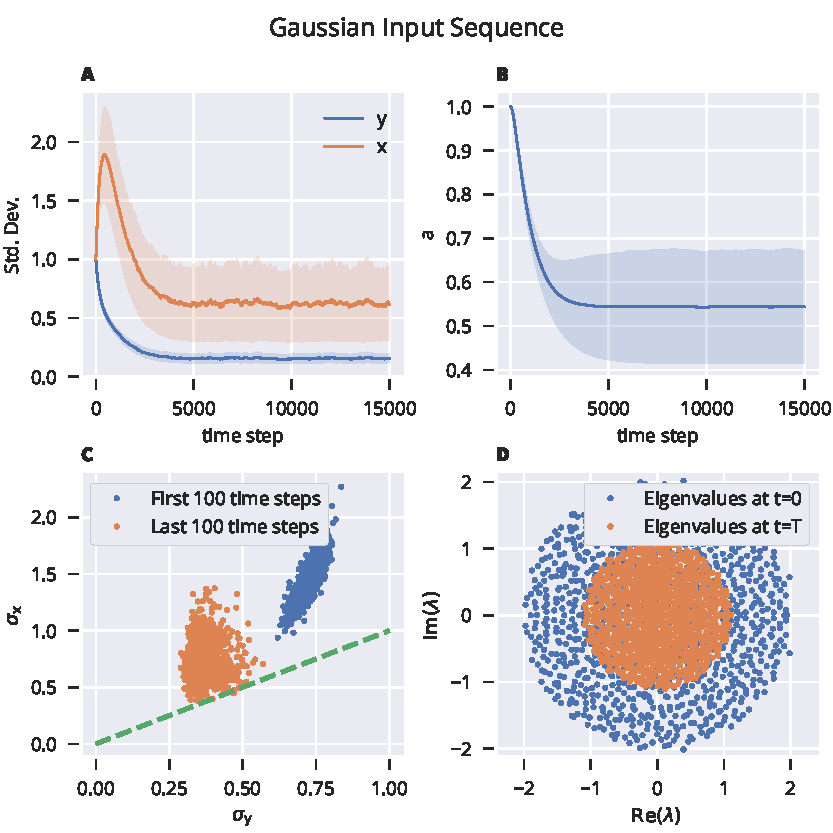
\includegraphics{../../plots/alternative_mech/composite.pdf}
	\caption{Results for $u$ drawn from a Gaussian distribution with zero mean, $1/4$ standard deviation, $R=1$ and $\sigma_{\rm W}=2$. Other parameters as in Table \ref{tab:params}. {\bf A}: Standard deviations (trailing average over time) of neural activities and membrane potentials. Shaded region denotes standard deviation over the neural population. {\bf B}: Gain mean and standard deviation over the neural population. {\bf C}: Standard deviations of membrane potentials versus standard deviations of activities. Each point represents a neuron. {\bf D}: Eigenvalues of $a_i W_{ij}$.}
	\label{fig:results_gaussian_sequ}
\end{figure}

\begin{figure}[ht]
	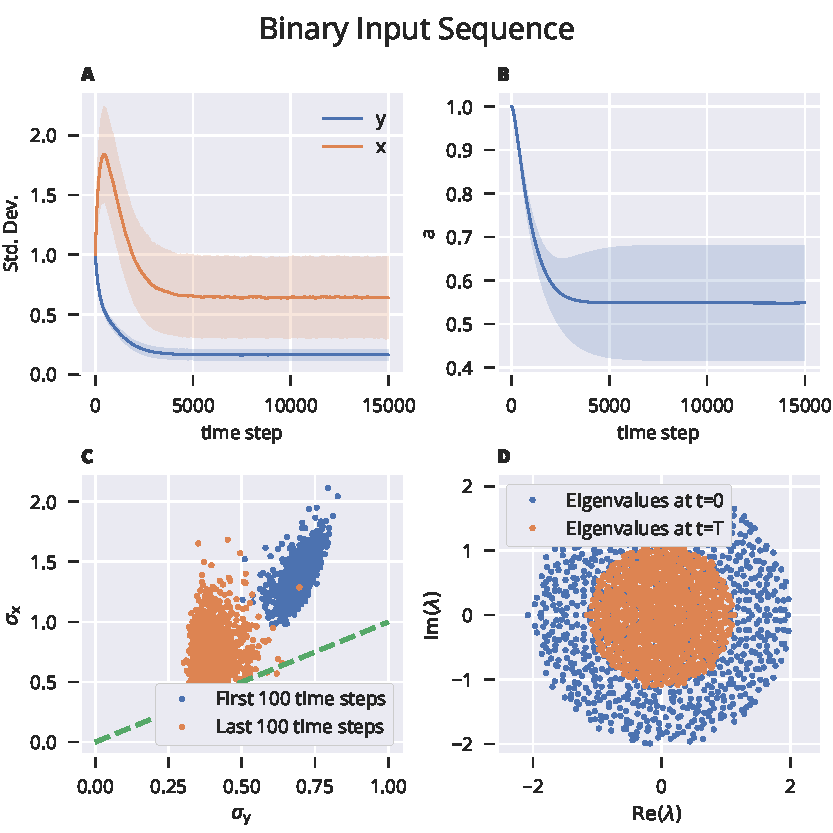
\includegraphics{../../plots/alternative_mech/composite_binary_sequ.pdf}
	\caption{Results as presented in Fig.~\ref{fig:results_gaussian_sequ}, for $u$ drawn from a symmetric binary distribution, $u(t) \in (-1/4,1/4)$.}
	\label{fig:results_binary_sequ}
\end{figure}

\begin{figure}[ht]
	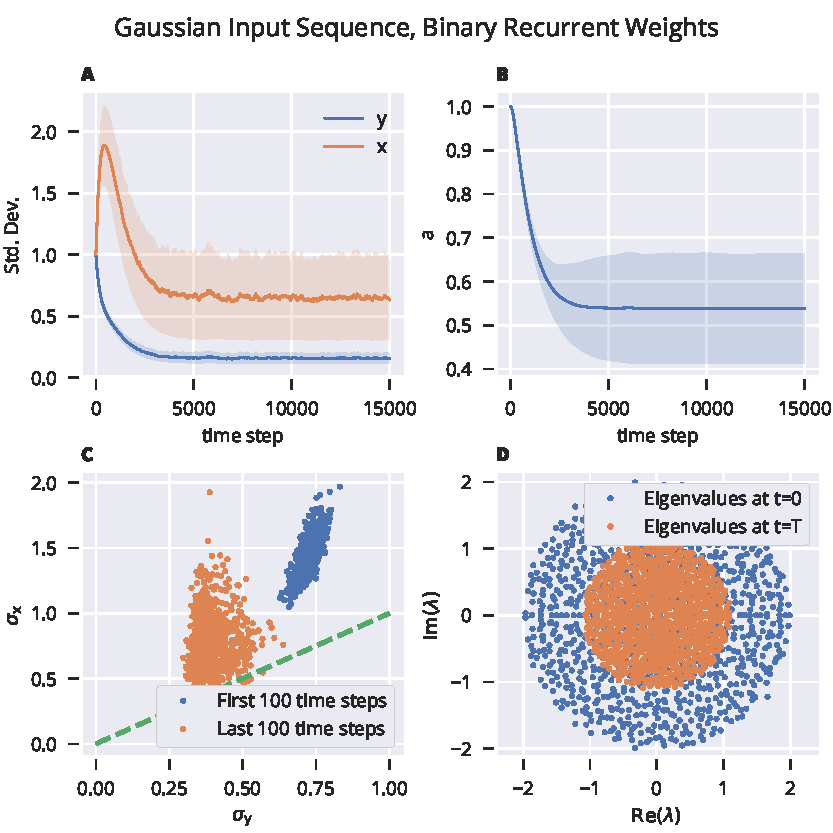
\includegraphics{../../plots/alternative_mech/composite_binary_matrix.pdf}
	\caption{Results as presented in Fig.~\ref{fig:results_gaussian_sequ}, for $W_{ij}$ drawn from a binary distribution.}
	\label{fig:results_binary_matrix}
\end{figure}

\begin{figure}[ht]
	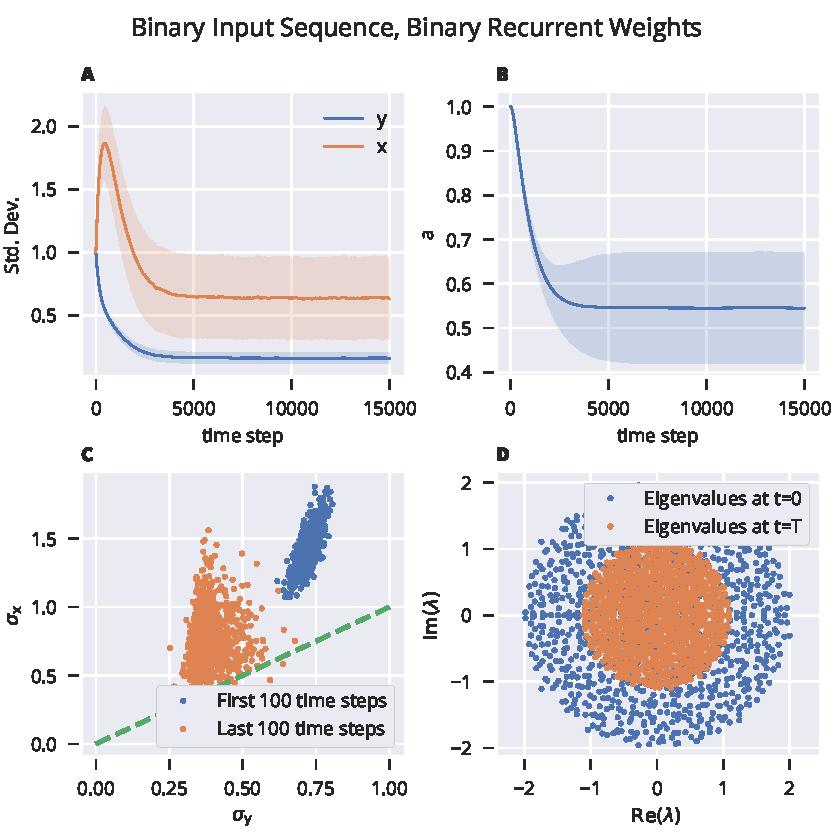
\includegraphics{../../plots/alternative_mech/composite_binary_matrix_binary_sequence.pdf}
	\caption{Results as presented in Fig.~\ref{fig:results_gaussian_sequ}, for $W_{ij}$ drawn from a binary distribution and $u$ drawn from a binary distribution, $u(t) \in (-1/4,1/4)$.}
	\label{fig:results_binary_matrix_binary_sequence}
\end{figure}


%%%%%%%%%%%%%%%%%%%%%%%%%%%%%%%%%%%%%%%%%%%%%%%%%%%%%%%
%\bibliographystyle{humannat}
%\bibliography{schubert_echo}
%%%%%%%%%%%%%%%%%%%%%%%%%%%%%%%%%%%%%%%%%%%%%%%%%%%%%%%

\end{document}